%!Tex Root = ../Tutorat2.tex
% ./Packete.tex
% ./Design.tex
% ./Deklarationen.tex
% ./Aufgabe1.tex
% ./Aufgabe2.tex
% ./Bonus.tex

\section{Task 3}

\setcounter{task}{1}

\begin{frame}{Task 3}{Bonus Practice\vspace{0.5cm}}
  \begin{itemize}
    \item We see from the table that the period P is 30, and we can use 3 as the frame f. Since this task set is a small one, we can derive a feasible schedule graphically...
  \end{itemize}
  \begin{figure}
    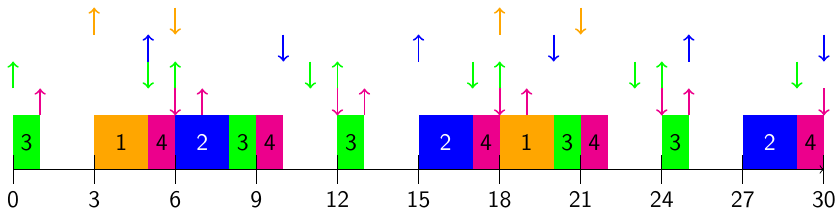
\includegraphics[width=0.7\paperwidth]{./figures/task3_schedule.png}
    \caption{Schedule for Task 3}
  \end{figure}
\end{frame}
